\section{Implementation}\label{sec:4}

This section maps the architecture in \S\ref{sec:3} to concrete repository artifacts.
The implementation is organized around four execution boundaries:
\begin{enumerate}[leftmargin=*]
  \item role-specific agents own mutable candidate and job state;
  \item a read-only Matchmaking agent ranks immutable snapshots;
  \item the React portals expose candidate, employer, and admin workflows; and
  \item offline assets reproduce the reported evaluation numbers.
\end{enumerate}
Figure~\ref{fig:8} shows the runtime matching path; \S\ref{sec:5} defines the scores and \S\ref{sec:6} reports outcomes.

\begin{JFigure}{../figures/Fig8.png}
\vspace{1\baselineskip}
\figcap{8}{Implementation of the matching pipeline: retrieval (exhaustive or ANN primary; lexical benchmark-only), composite scoring with six weighted components, feasibility constraints, optional fusion/calibration/feedback boost/auto-strategy, and structured explanation fork (rule default, LLM optional) consumed by portal cards and drawer.}
\end{JFigure}

\subsection{Backend implementation}\label{sec:4-backend}

\leadpara{Deployment shape.}
The backend is a single FastAPI process built by \texttt{backend/gateway/app.py} and wired through \texttt{bootstrap.py}.
Routers mount at the root rather than under a global \texttt{/api} prefix.
Session cookies use \texttt{jm\_session} with a 7-day max age, and an optional \texttt{ReadOnlyMiddleware} blocks writes when \texttt{read\_only=true}.
The committed default listen address is \texttt{0.0.0.0:8001}.

\begin{JTable}
\caption{Backend implementation map.}
\label{tab:implementation-backend}
\scriptsize
\begin{tabular}{@{}p{0.16\linewidth}p{0.34\linewidth}p{0.42\linewidth}@{}}
\toprule
Layer & Repository artifact & Responsibility \\
\midrule
Gateway & \path{gateway/app.py}, \path{gateway/routes/*} & Builds the FastAPI app and exposes \texttt{/auth}, \texttt{/agents}, \texttt{/candidates}, \texttt{/jobs}, \texttt{/match/*}, \texttt{/similar}, \texttt{/feedback}, \texttt{/system}, and \texttt{/real-jobs}. \\
Container & \path{bootstrap.py} & Constructs agents, stores, event bus, seeded corpora, and optional live-job snapshot replacement. \\
Candidate agent & \path{agents/candidate_agent.py}, \path{hooks/parser.py} & Parses résumés, versions candidate snapshots, embeds canonical text, and upserts to \texttt{candidates\_collection}. \\
Employer agent & \path{agents/employer_agent.py} & Registers job postings, embeds descriptions, upserts to \texttt{jobs\_collection}, and supports \texttt{replace\_corpus} for bulk refresh. \\
Matchmaking agent & \path{agents/matchmaking_agent.py} & Reads snapshots, runs retrieval/scoring, emits \texttt{MATCH\_COMPLETED}, and never mutates profile stores. \\
Scoring core & \path{core/scoring.py}, \path{matchmaking_scoring.py}, \path{component_scores.py} & Implements semantic, skill, title, experience, compensation, remote, multimodal, and composite scores. \\
Optional rankers & \path{core/rrf.py}, \path{fusion.py}, \path{calibration.py}, \path{feedback_boost.py}, \path{cross_encoder_rerank.py} & Adds ensemble fusion, learned fusion, Platt calibration, user-feedback deltas, and cross-encoder reranking when enabled. \\
Explanations & \path{core/match_explanation.py}, \path{core/explain.py} & Produces structured fit signals, score breakdowns, and rule-based explanation bullets for portal cards and drawers. \\
Stores & \path{stores/factory.py}, \path{auth/store.py}, \path{feedback_store.py}, \path{candidate_activity_store.py} & Selects Chroma/Qdrant, persists roles and sessions, stores feedback, saved jobs, applications, and activity rows. \\
\bottomrule
\end{tabular}
\normalsize

\end{JTable}

\leadpara{Matching execution path.}
At runtime, the owning agent embeds and registers each profile snapshot, then emits a profile-update event.
The Matchmaking agent consumes only snapshots, retrieves an exhaustive or ANN-filtered candidate set, rescales the requested component scores, attaches explanations, and returns a top-$K$ list.
Lexical BM25/TF--IDF retrieval is kept for offline baselines and is not the portal default.

\leadpara{Live job refresh.}
The optional live-feed path is deliberately isolated from the offline corpus.
\path{core/real_jobs_sync.py} performs paginated upstream \texttt{GET} requests, normalizes external fields, deduplicates identifiers, and writes \path{data/jobs_live.json}.
\path{services/real_jobs_service.py} then calls \texttt{EmployerAgent.replace\_corpus} and may re-embed candidates and jobs through \texttt{reindex\_all}.
The API surface is \texttt{GET} \path{/real-jobs/status} and \texttt{POST} \path{/real-jobs/sync}; the CLI equivalent is \texttt{python} \path{backend/scripts/sync_real_jobs_once.py}.

\leadpara{Authentication and route ownership.}
The roles are \texttt{candidate}, \texttt{employer}, and \texttt{admin}.
Gateway dependencies enforce ownership for profile-scoped routes:
\begin{itemize}[leftmargin=*]
  \item \textbf{Candidate:} \texttt{/candidates/me/*}, résumé upload, saved jobs, applications, and \texttt{/similar/jobs/*}.
  \item \textbf{Employer:} \texttt{/jobs/mine/*}, description upload/parse, applications for owned jobs, and \texttt{/similar/candidates/*}.
  \item \textbf{Admin:} demo reset and system-level inspection routes.
\end{itemize}
Matching and agent telemetry endpoints remain callable without role checks so the admin console and integration tests can invoke them directly.

Table~\ref{tab:workflows} summarizes the main end-to-end user flows and the API/agent path behind each one.

\begin{JTable}
\caption{Primary user-facing workflows by role ($K{=}10$ composite matching unless noted).}
\label{tab:workflows}
\small
\begin{tabular}{@{}p{0.11\linewidth}p{0.17\linewidth}p{0.22\linewidth}p{0.38\linewidth}@{}}
\toprule
Role & Portal route & User goal & API / agent path \\
\midrule
Candidate & \texttt{/candidate/onboarding} & Upload resume, review extraction, create profile & \texttt{POST /candidates/upload-resume} $\rightarrow$ \texttt{PUT /candidates/me} $\rightarrow$ Candidate agent registers snapshot + embedding \\
Candidate & \texttt{/candidate/profile} & Edit skills, experience, pay, remote prefs & \texttt{GET/PUT /candidates/me}; quality via \texttt{POST /candidates/quality-check} \\
Candidate & \texttt{/candidate/matches} & View ranked jobs, filter, explain scores & \texttt{POST /match/candidate-to-jobs} (composite); profile readiness gate before search \\
Candidate & \texttt{/candidate/saved} & Saved jobs and applications & \texttt{GET/PUT /candidates/me/saved-jobs}; \texttt{POST /candidates/me/applications} \\
Employer & \texttt{/employer/jobs} & Import JD, post/edit/close roles & \texttt{POST /jobs/upload-description} or \texttt{/parse-description} $\rightarrow$ \texttt{POST /jobs} or \texttt{PUT /jobs/mine/\{id\}} $\rightarrow$ Employer agent \\
Employer & \texttt{/employer/matches} & Rank candidates for a owned job & \texttt{POST /match/job-to-candidates} (composite); job ownership required \\
Employer & \texttt{/employer/applications} & Review applicants per posting & \texttt{GET /jobs/mine/applications} (SQLite activity store) \\
Admin & \texttt{/admin/console} & Monitor agents, run matches, inspect fairness & \texttt{GET /agents/status}, \texttt{/agents/events/recent}, \texttt{/system/config}; optional \texttt{/match/*}, \texttt{/system/fairness}, \texttt{POST /real-jobs/sync} when live feed enabled \\
\bottomrule
\end{tabular}
\normalsize
\par\vspace{0.4em}
\footnotesize{All authenticated routes use cookie sessions (\texttt{withCredentials}) and FastAPI \texttt{require\_role} guards. Match endpoints invoke the Matchmaking agent read-only over snapshots.}

\end{JTable}

\subsection{Frontend implementation}\label{sec:4-frontend}

The UI is a React~19 single-page application built with Vite.
All portals use axios with session cookies and role guards in \texttt{App.jsx}; shared navigation and layout live in \texttt{PortalShell}.

\begin{itemize}[leftmargin=*]
  \item \textbf{Candidate portal:} \path{/candidate/onboarding}, \path{/candidate/profile}, \path{/candidate/matches}, and \path{/candidate/saved}. Profile saves dispatch \texttt{jobmatch:profile-updated}; match and saved-job views refetch on that signal. Explanation surfaces are \texttt{MatchExplainability} and \texttt{MatchDetailsDrawer}.
  \item \textbf{Employer portal:} \path{/employer/jobs}, \path{/employer/matches}, and \path{/employer/applications}. The job editor and upload flow call \path{/jobs/mine/*}; reverse matching uses \texttt{mode=job\_to\_candidates}.
  \item \textbf{Admin console:} \path{/admin/console}. Panels show agent status, recent events, system config, manual match controls, recent results in \texttt{localStorage}, and the fairness summary from \texttt{GET} \path{/system/fairness}. Live sync is available through the API and CLI, but no dedicated admin button is wired.
  \item \textbf{Error routes:} full-screen 404/502/unknown-error pages distinguish client routing failures from upstream outages.
\end{itemize}

Figure~\ref{fig:10} shows the portal surfaces that invoke the matching pipeline in Figure~\ref{fig:8}.
Screenshots use the demo corpus and default composite strategy; they demonstrate the research prototype UI, not a usability study.

\begin{figure}[p]
\centering
\begin{minipage}{0.98\linewidth}
\centering
\JFigFramed{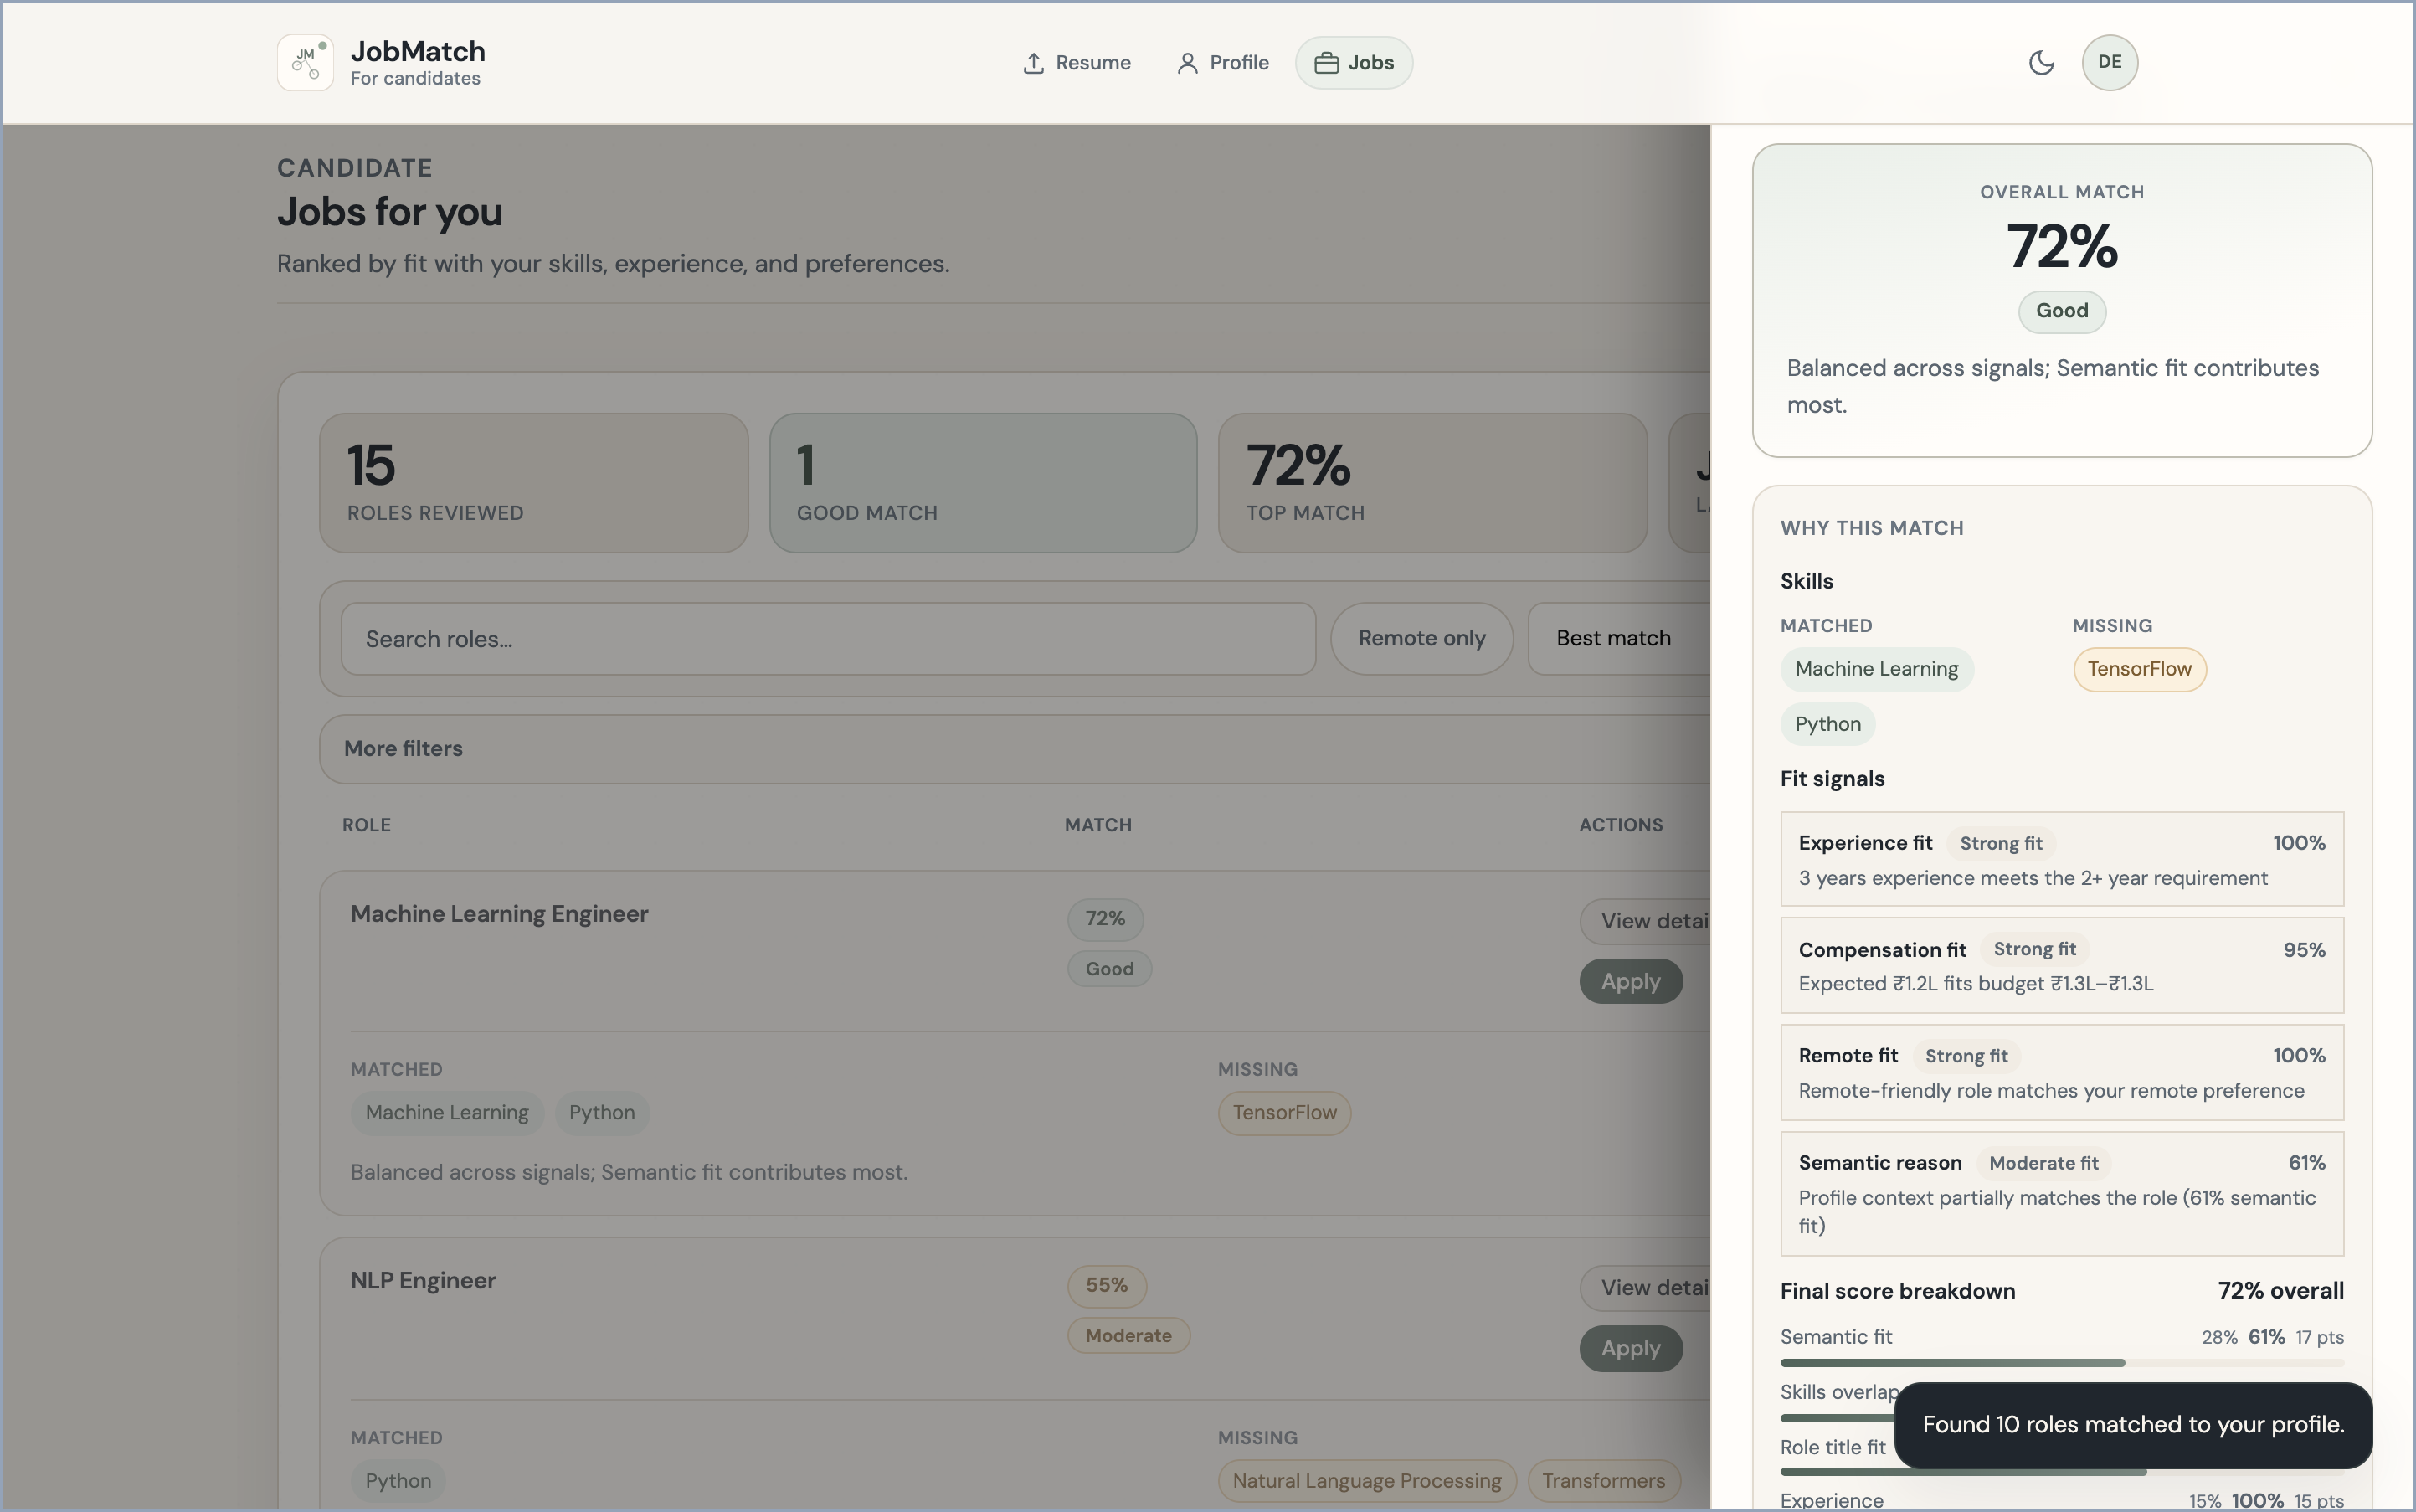
\includegraphics[width=0.99\linewidth,height=0.30\textheight,keepaspectratio]{../figures/screenshots/ui-candidate-matches.png}}\\[3pt]
{\small (a) Candidate job matches}
\end{minipage}\\[0.65\baselineskip]
\begin{minipage}{0.98\linewidth}
\centering
\JFigFramed{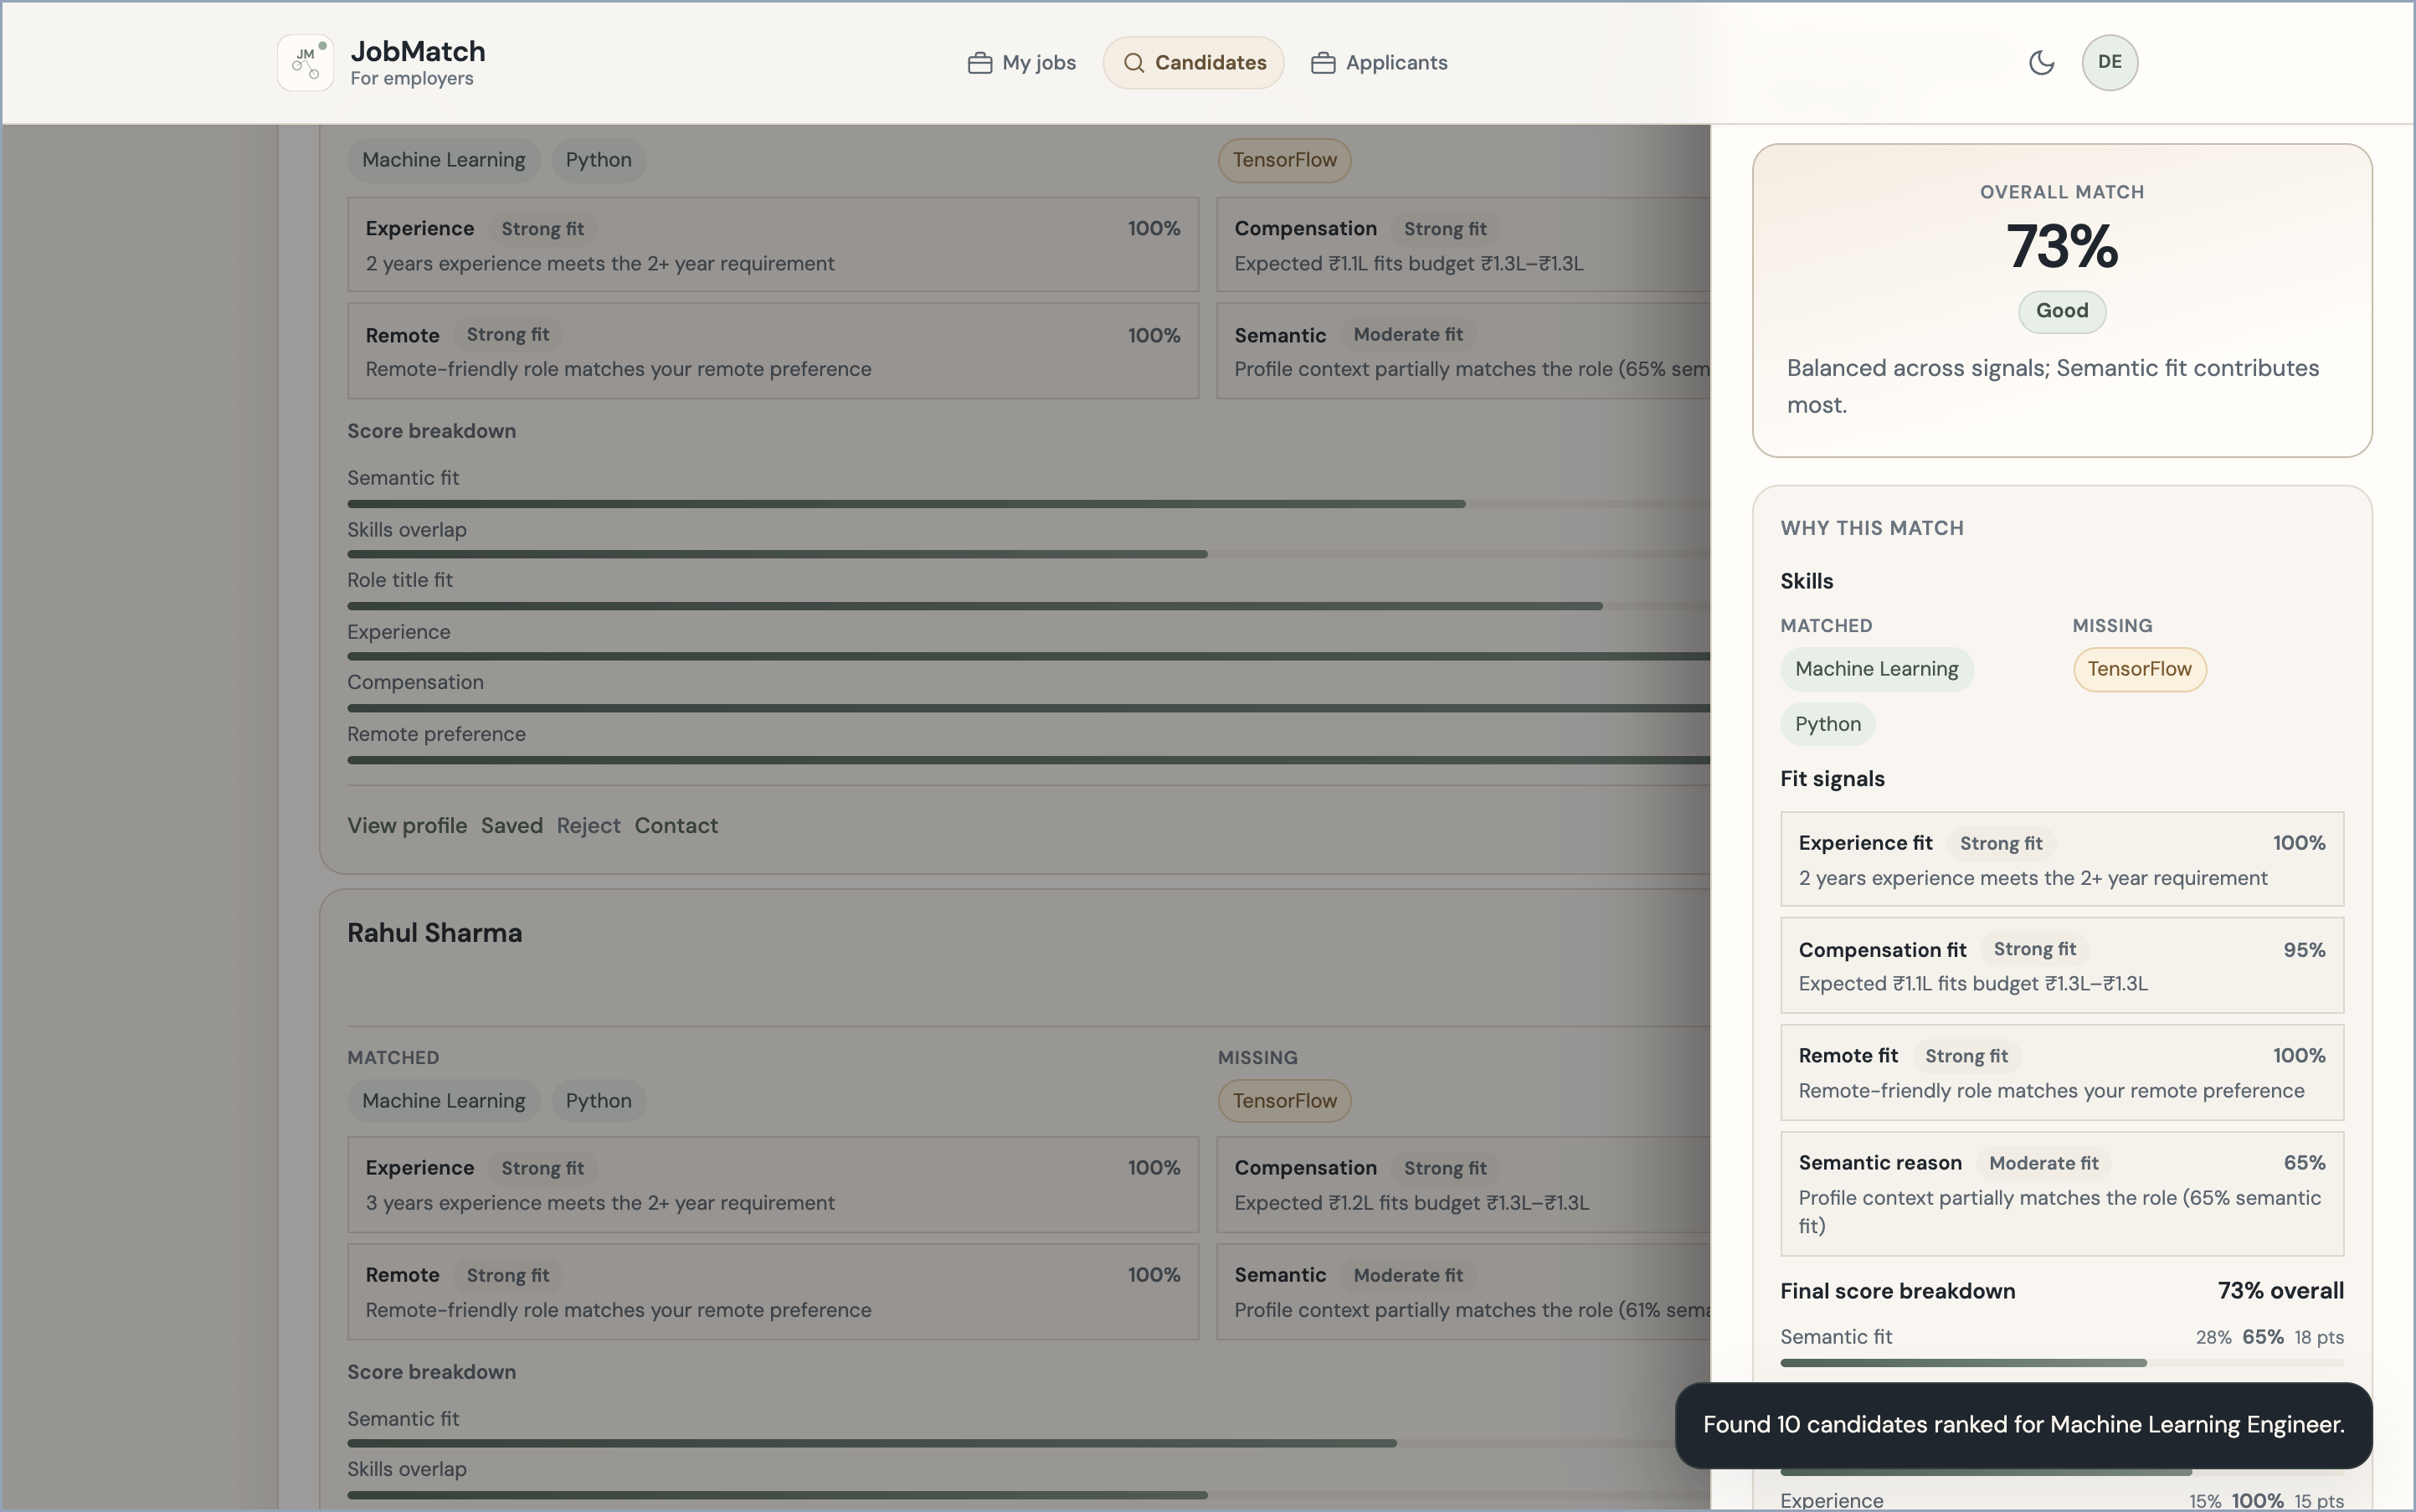
\includegraphics[width=0.99\linewidth,height=0.30\textheight,keepaspectratio]{../figures/screenshots/ui-employer-matches.png}}\\[3pt]
{\small (b) Employer reverse search}
\end{minipage}\\[0.65\baselineskip]
\begin{minipage}{0.98\linewidth}
\centering
\JFigFramed{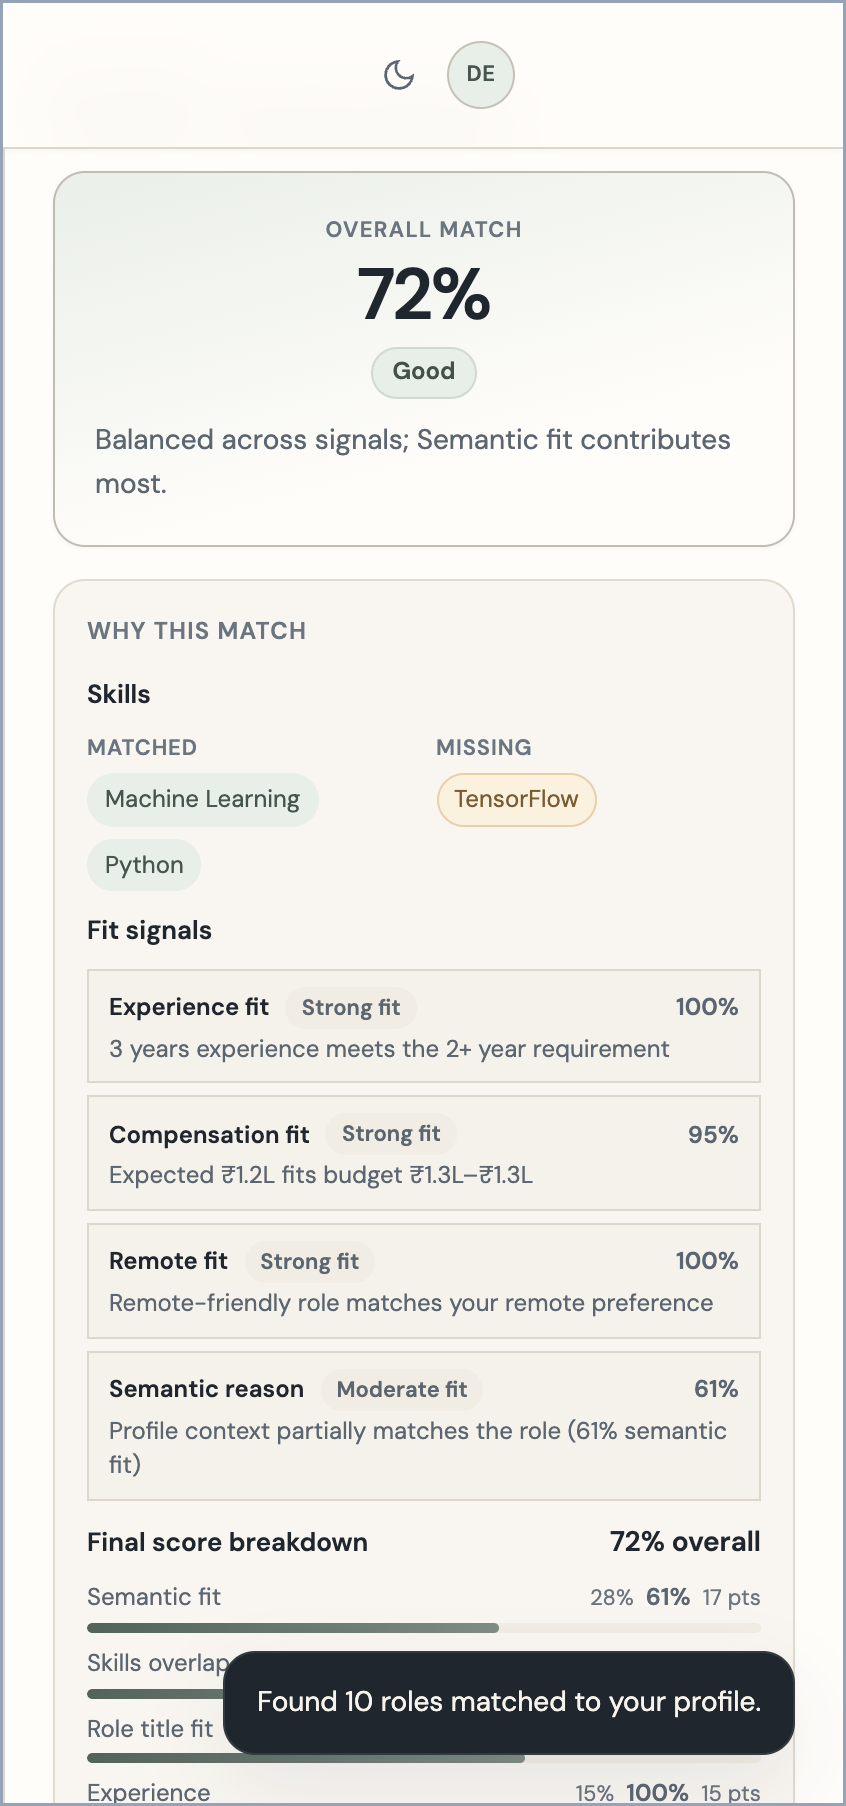
\includegraphics[width=0.99\linewidth,height=0.36\textheight,keepaspectratio]{../figures/screenshots/ui-score-breakdown.png}}\\[3pt]
{\small (c) Composite score breakdown}
\end{minipage}
\figcap{10}{Portal implementation backing the workflows in Figures~\ref{fig:6}--\ref{fig:7} and the matching pipeline in Figure~\ref{fig:8}: (a) candidate job matches with explanation drawer; (b) employer reverse candidate search for an owned posting; (c) composite score breakdown and skill alignment (portal default strategy, top-$K{=}10$).}
\end{figure}

\subsection{Data contracts}\label{sec:4-data}

Contracts are Pydantic models in \texttt{backend/contracts/}.
The key invariant is that the Matchmaking agent scores snapshots, not editable portal records.
Table~\ref{tab:implementation-contracts} lists the objects that cross the boundary between agents, stores, and portals.

\begin{JTable}
\caption{Primary data contracts used by the Matchmaking agent and portals.}
\label{tab:implementation-contracts}
\scriptsize
\begin{tabular}{@{}p{0.19\linewidth}p{0.34\linewidth}p{0.39\linewidth}@{}}
\toprule
Contract & Key fields & Where it is used \\
\midrule
Candidate snapshot & \begin{itemize}[leftmargin=*,nosep]
  \item identity: \texttt{id}, \texttt{name}
  \item profile: \texttt{skills}, experience, salary, remote preference
  \item trace: \texttt{version}, text hash, \texttt{embedding}
\end{itemize} & Created by the Candidate agent after resume/profile updates; scored by the Matchmaking agent. \\
Job snapshot & \begin{itemize}[leftmargin=*,nosep]
  \item posting: title, description, required/preferred skills
  \item fit constraints: experience, budget, remote policy
  \item metadata: company, link, location, source, version, hash, embedding
\end{itemize} & Created by the Employer agent from portal jobs, snapshots, or live feeds; vector metadata supports filters and admin inspection. \\
Match result & \begin{itemize}[leftmargin=*,nosep]
  \item target: \texttt{target\_id}, label, rank
  \item scores: similarity, six components, \texttt{final\_score}
  \item context: skills, metadata, constraints, optional explanation
\end{itemize} & Returned to candidate and employer portals as the ranked item row. \\
Match explanation & \begin{itemize}[leftmargin=*,nosep]
  \item matched and missing skills
  \item four fit signals
  \item weighted score breakdown
\end{itemize} & Drives the explanation drawer and score-breakdown UI. \\
Match response & \begin{itemize}[leftmargin=*,nosep]
  \item \texttt{session\_id}, direction, strategy
  \item corpus counters and agent versions
  \item results and optional rerank diagnostics
\end{itemize} & Wraps each matching call so tests and portals can inspect strategy and corpus context. \\
\bottomrule
\end{tabular}
\normalsize

\end{JTable}

\leadpara{Feedback and events.}
\texttt{FeedbackStore} records user, target, action, optional context, role, and timestamp.
Match-scoped actions are \texttt{save}, \texttt{dismiss}, and \texttt{apply}; broader actions include \texttt{contact}, \texttt{reject}, and \texttt{not\_interested}.
Feedback never rewrites embeddings and affects ranking only when \texttt{use\_feedback\_boost=true}.
Agent events cover profile updates, corpus bootstrap, match requests, and match completions; emitted event names are surfaced in the admin event strip.

\subsection{Libraries and runtime defaults}\label{sec:4-libraries}

JobMatch ships as one backend process plus one static SPA bundle; there is no inter-service RPC layer beyond the in-process event bus.
Only dependencies declared in the repository are listed here:
\begin{itemize}[leftmargin=*]
  \item \textbf{Backend framework:} FastAPI~0.129, Uvicorn~0.29, Pydantic~2.9, and \texttt{pydantic-settings}.
  \item \textbf{Backend data/retrieval:} NumPy~1.26, Sentence-Transformers~5.1, ChromaDB~0.4.24, and optional Qdrant client~1.12.
  \item \textbf{Backend utilities:} HTTPX, Passlib/bcrypt, \texttt{python-multipart}, \texttt{python-dotenv}, pdfplumber, \texttt{email-validator}, \texttt{itsdangerous}, and optional \texttt{tiktoken}~0.8.
  \item \textbf{Storage/frontend:} SQLite through Python \texttt{sqlite3}; React~19, React DOM, React Router~7, axios~1.7, Vite~6, and \texttt{@vitejs/plugin-react}.
\end{itemize}

\subsection{Parameter settings}\label{sec:4-params}

Table~\ref{tab:implementation-params} separates portal defaults, API defaults, optional branches, and live-job gates.
The portal default is intentionally conservative: fixed composite scoring, rules-based explanations, no calibration, no feedback boost, no cross-encoder rerank, and no automatic strategy switch.

\begin{table}[!htbp]
\centering
\caption{Runtime and evaluation defaults.}
\label{tab:implementation-params}
\scriptsize
\begin{tabular}{@{}p{0.24\linewidth}p{0.30\linewidth}p{0.38\linewidth}@{}}
\toprule
Setting group & Default value & Notes \\
\midrule
Embedding and vector store & \begin{itemize}[leftmargin=*,nosep]
  \item model: \texttt{all-MiniLM-L6-v2}
  \item dimension: 384
  \item default store: \path{vector_store=chroma}
\end{itemize} & Qdrant is available through the same store interface; Chroma uses cosine space by default. \\
Portal match request & \begin{itemize}[leftmargin=*,nosep]
  \item \texttt{topK=10}; exhaustive retrieval
  \item composite, cosine, Jaccard skills
  \item rules explanations
\end{itemize} & Used by \path{DEFAULT_CANDIDATE_MATCH} and \path{DEFAULT_EMPLOYER_MATCH} on the demo corpus. \\
API/evaluation request & \begin{itemize}[leftmargin=*,nosep]
  \item \path{top_k=5}
  \item \path{candidate_pool=120}
  \item exhaustive retrieval
\end{itemize} & Offline evaluation and regression tests use $K{=}5$ unless a driver overrides \texttt{--top-k}. \\
Composite weights & \begin{itemize}[leftmargin=*,nosep]
  \item semantic 28\%; skills 27\%
  \item title 10\%; experience 15\%
  \item compensation 10\%; remote 10\%
\end{itemize} & Matches Eq.~\ref{eq:composite} and the portal-default ablation. \\
Fusion and calibration & \begin{itemize}[leftmargin=*,nosep]
  \item \path{Settings.rrf_k=60}
  \item \path{fusion.json}
  \item \path{calibration.json}: $a{\approx}0.298$, $b{\approx}{-}2.116$
\end{itemize} & Available for evaluation/experiments; calibration is disabled in portal defaults. \\
Explanation labels & \begin{itemize}[leftmargin=*,nosep]
  \item Strong $\geq 0.85$
  \item Good $\geq 0.65$
  \item Moderate $\geq 0.45$; else Weak
\end{itemize} & Rule bullets additionally use title and semantic narrative cutoffs. \\
Constraint and feedback branches & \begin{itemize}[leftmargin=*,nosep]
  \item experience-gap penalty: $0.65$
  \item save $+0.04$; apply $+0.06$
  \item dismiss $-0.06$
\end{itemize} & Applied only when constraints or feedback boost are enabled. \\
Cross-encoder branch & \begin{itemize}[leftmargin=*,nosep]
  \item rerank pool: 20
  \item \path{enable_cross_encoder_rerank=false}
\end{itemize} & Disabled in production settings and portal defaults. \\
Live-job sync & \begin{itemize}[leftmargin=*,nosep]
  \item \path{REAL_JOBS_ENABLE=false}
  \item page limit 100; timeout 30s
  \item output: \path{data/jobs_live.json}
\end{itemize} & Daily batch pre-syncs only when live jobs are enabled. \\
\bottomrule
\end{tabular}
\normalsize

\end{table}

\subsection{Reproducibility}\label{sec:4-benchmarks}

The evaluation path uses frozen data and scripted drivers rather than portal state.
Table~\ref{tab:implementation-repro} lists the artifacts needed to reproduce the paper-facing runs.
ANN shortlist latency is summarized separately in Table~\ref{tab:latency} from the committed \texttt{phase11\_summary.csv}.

\begin{table}[!htbp]
\centering
\caption{Reproducibility assets and verification paths.}
\label{tab:implementation-repro}
\scriptsize
\begin{tabular}{@{}p{0.24\linewidth}p{0.34\linewidth}p{0.34\linewidth}@{}}
\toprule
Category & Files or commands & Purpose \\
\midrule
Frozen corpus & \begin{itemize}[leftmargin=*,nosep]
  \item \path{data/cvs.json}
  \item \path{data/jobs.json}
  \item \path{data/eval_pairs.json}
\end{itemize} & Provides 30 résumés, 15 jobs, and 47 graded query--document relevance pairs. \\
Auxiliary assets & \begin{itemize}[leftmargin=*,nosep]
  \item fairness profiles and expected metrics
  \item fusion and calibration models
\end{itemize} & Stores fairness probes, expected metrics, learned fusion weights, and Platt calibration parameters. \\
Research mirror & \path{data/research/*} & Mirrors the corpus and manifest used by paper-facing export scripts. \\
Benchmark drivers & \begin{itemize}[leftmargin=*,nosep]
  \item comparison, ablation, paper tables
  \item significance, explainability, fairness
\end{itemize} & Recomputes ranking metrics, ablations, paper tables, significance tests, explainability checks, and fairness audit outputs. \\
Pipeline wrapper & \path{backend/scripts/run_research_pipeline.py} & Runs the orchestrated research pipeline with default \texttt{--top-k 5}. \\
Test runner & \begin{itemize}[leftmargin=*,nosep]
  \item \texttt{bash scripts/run\_tests.sh}
  \item backend: \texttt{pytest ../tests -q}
\end{itemize} & Runs Python unit/integration/benchmark tests plus frontend utility tests. \\
Regression gate & \path{tests/benchmarks/test_eval_regression.py} & Recomputes semantic and multimodal rankings and checks nDCG@5 against frozen expected metrics with $\pm 0.04$ tolerance. \\
Live-job contract tests & \begin{itemize}[leftmargin=*,nosep]
  \item \path{test_real_jobs_sync.py}
  \item \path{test_real_jobs_api.py}
\end{itemize} & Verifies normalization, pagination mock, snapshot I/O, status endpoint, and disabled-sync behavior. \\
\bottomrule
\end{tabular}
\normalsize

\end{table}
